\subsection{Database Design}
\subsubsection{Database Overview}
\begin{center}
  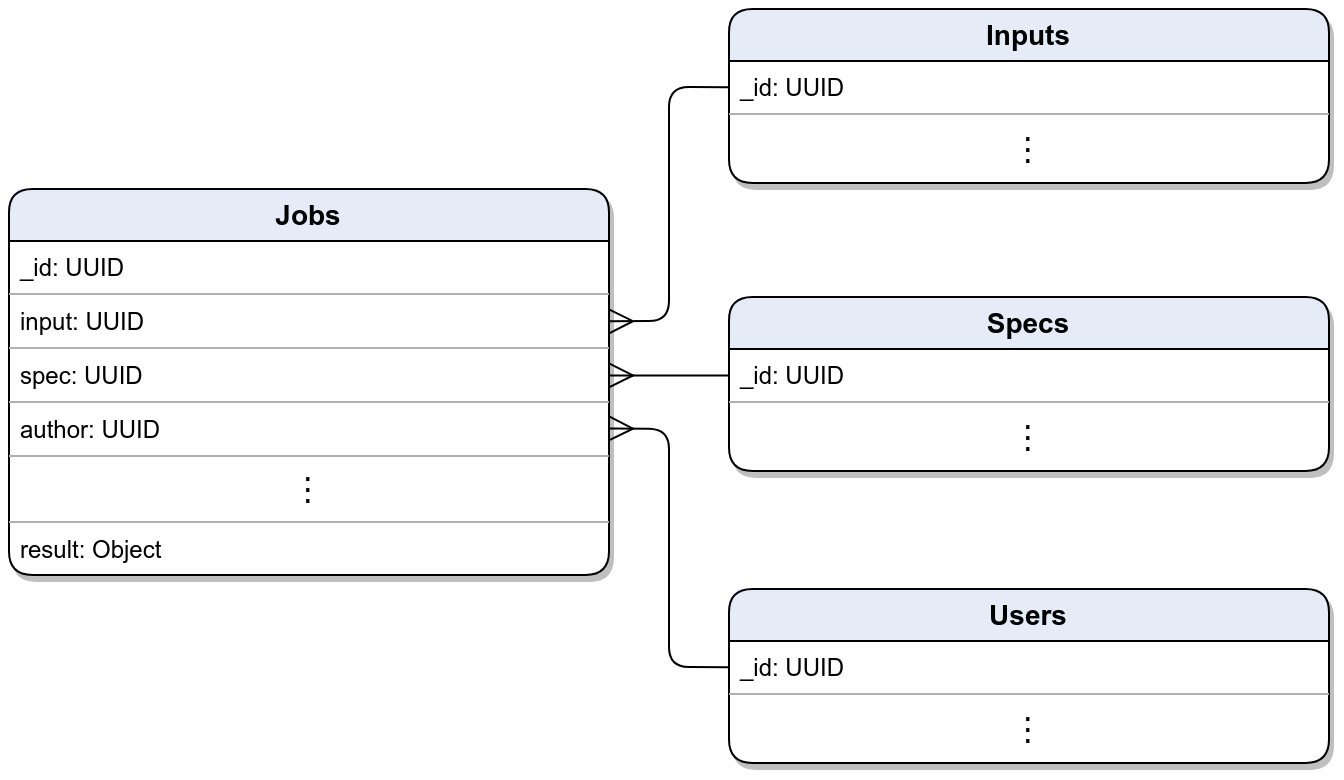
\includegraphics[width=\textwidth]{DatabaseOverview} \\[12pt]
\end{center}
The diagram above represents the database implementation that will be used in the server application at a high level---more detailed representations will follow in the sections below. Note that while this is an entity-relationship diagram, a type of diagram normally used to represent relational databases, a non-relational database (MongoDB) will be used for this application. The ERD, while an imperfect representation for a non-relational database, simply provides a convenient way of demonstrating the format in which information will be stored in collections and the ways in which these collections will relate to one another.\par
There are five collections that will be used to store all information in the database: Jobs, Inputs, Specs, Users, and Groups. The Jobs collection is at the core of the design, as jobs are where the action happens. This collection contains the UUID\textquotesingle s of each relevant document from other collections, metadata about each job, and, upon completion of the job, the resulting output from the analysis performed. The Inputs collection contains information about the WAV audio files to be processed by each job, including the location in which each of the files is stored on the server. The Specs collection holds information about how to process each job, namely, the list of parameters needed for each metric to be run. The Users and Groups collections contain information necessary in keeping track of users and groups.\par
The database is implemented using Mongoose, which allows for a schema-based object modeling approach to designing the MongoDB database and validating its documents. Mongoose\textquotesingle s capabilities play a vital role in the database implementation, as the object modeling features allow for inheritance between schemas, and this can be seen in both the Job and Spec models as shown in the next section.

\subsubsection{Jobs, Inputs, \& Specifications}
\begin{center}
  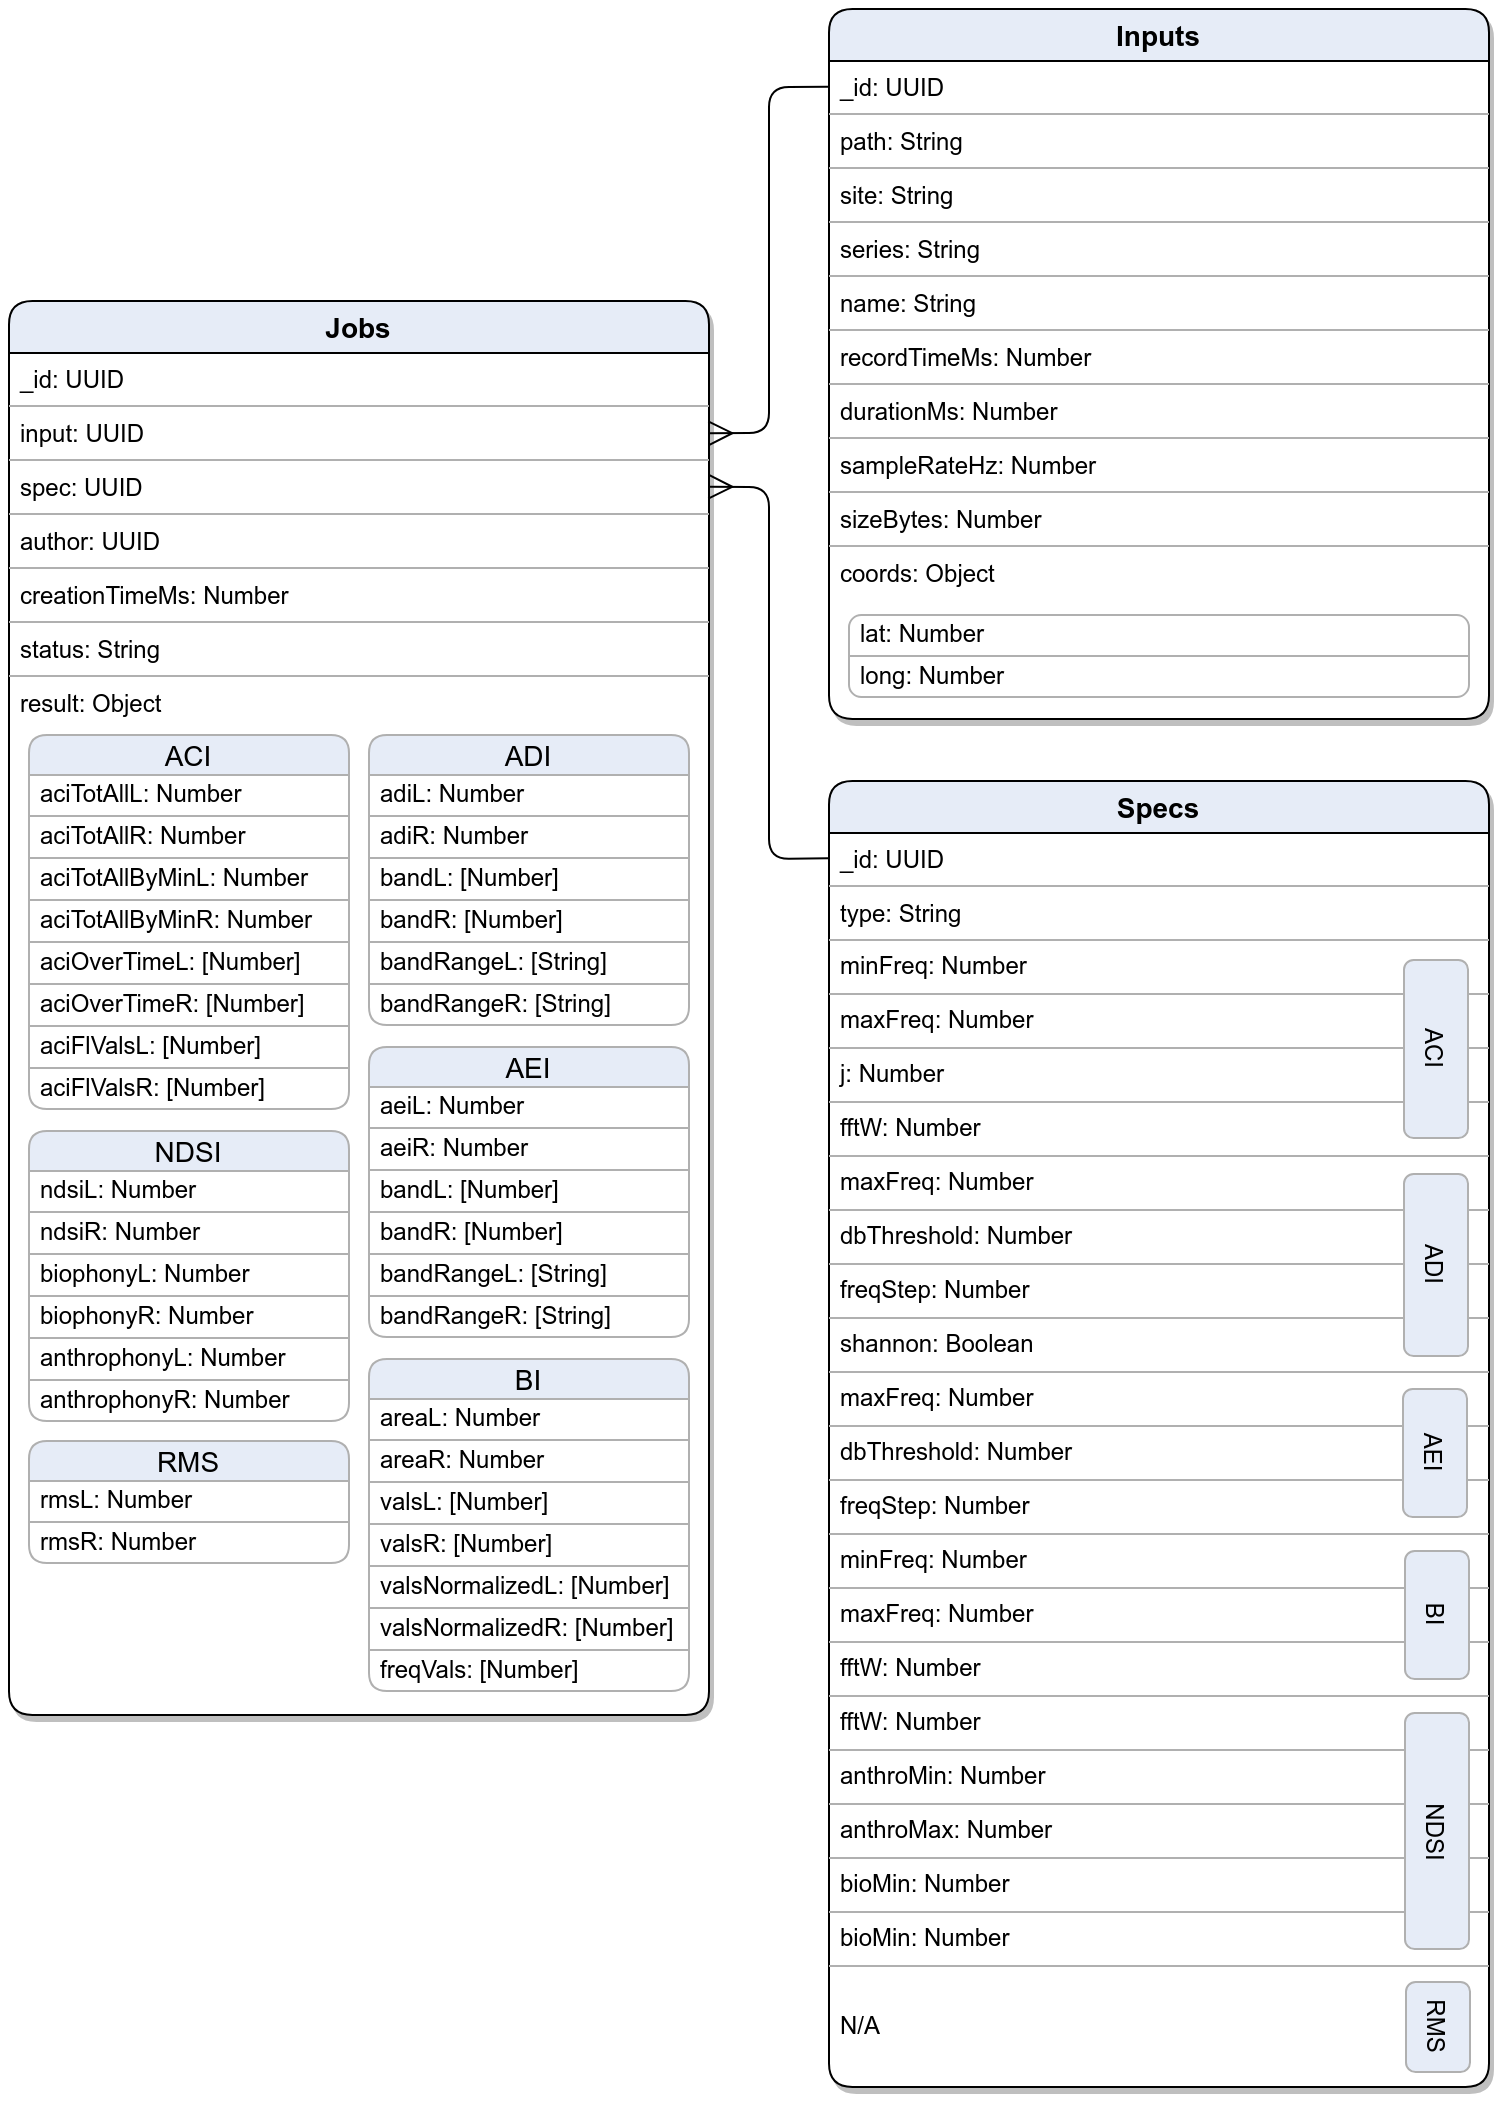
\includegraphics[width=\textwidth]{DatabaseJobs} \\[12pt]
\end{center}
It should be clear from the diagram that the database design is focused around the Jobs collection, and this makes sense given that jobs are where the action takes place. The Jobs collection connects to the Inputs, Specs, and Users collections via the UUID\textquotesingle s of a document from each of these being stored in each job document. Additionally, the metadata of when each job was initially created is stored in \codesnip{creationTimeMs}. The \codesnip{status} of each job is an enumerative String that may hold one of the following values: \codesnip{"queued"}, \codesnip{"processing"}, \codesnip{"finished"}, \codesnip{"failed"}, or \codesnip{"cancelled"}. Upon the completion of the processing phase of a job (marked by a \codesnip{status} of \codesnip{"finished"}), the \codesnip{result} Object will be populated with the results of each \codesnip{type} of job. The possibilities can be seen above.\par
It is important to note the way in which the different types of jobs are able to be stored in the same collection, as differences in job type contain variations on the Objects stored in the \codesnip{result}. This is done by a Mongoose\textquotesingle s feature called a \textit{discriminator}. Discriminators are what enable inheritance between different Mongoose models, and in both the Job and Spec models, they are used to define each ``child'' model. For example, while we have the ``parent'' model of Job, we also have the AciJob, NdsiJob, and so on, that inherit from it. Likewise, a similar approach is taken with the Spec models. The result is that each child model is stored in the same collection as those that share the same parent, and this provides the benefit of being able to regard only that collection when pulling information from the database.\par
The Specs collection represents the parameters used in each job. These parameters are specific to each metric being calculated by the job. Keeping these parameters separate from each job allows for reusability in the sense that if a user wants to run the same parameters on multiple inputs, all he or she must do is create an identical job with a different input, rather than defining the parameters each time.

\subsubsection{Users \& Groups}
\begin{center}
  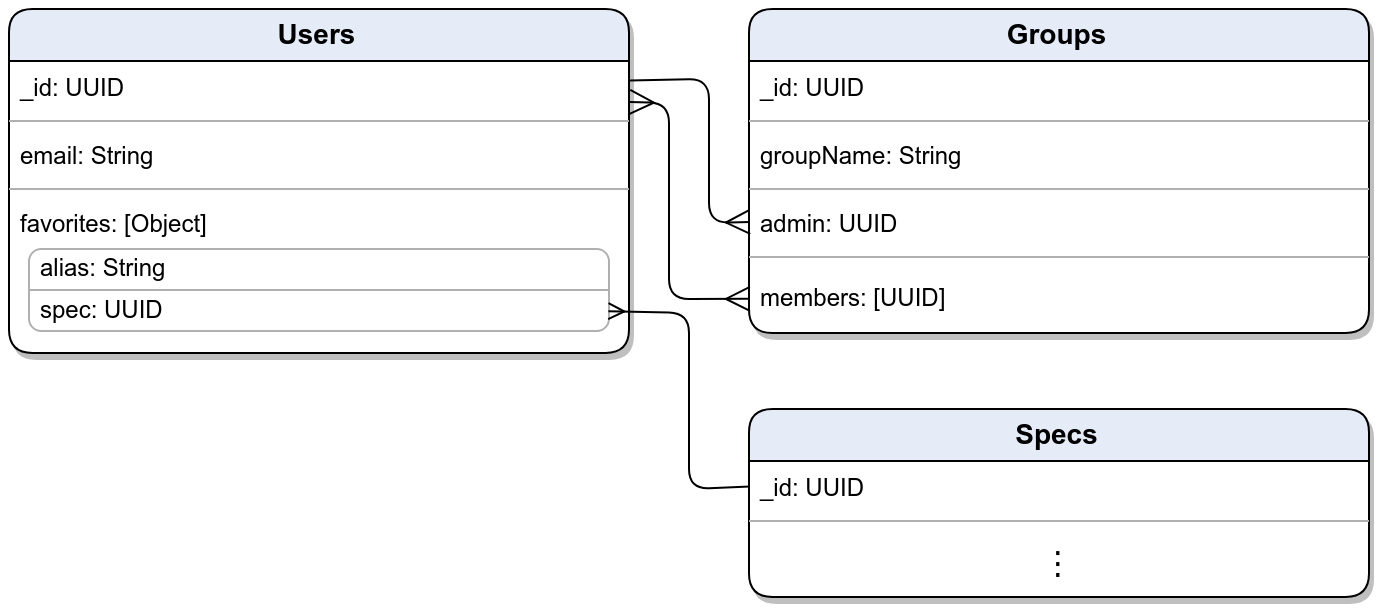
\includegraphics[width=\textwidth]{DatabaseUsers} \\[12pt]
\end{center}
While the heavy-lifting of user authentication will be handled by AWS Cognito, it can still be useful to store some pieces of user data in the database. For example, once authenticated, a user then has access to his or her list of favorite specifications, which can be used in the client application to simplify the creation of new jobs. The Users collection is where this kind of information will be stored.\par
Users can also be a part of one or more groups, or create a group. If a user creates a group, they are added as the admin of the group. An admin of a group can then add more users to also be admins. Groups have a list of members as well, and this references the Users collection.\par
